\chapter{Deuteronomy 2}

\begin{figure}
  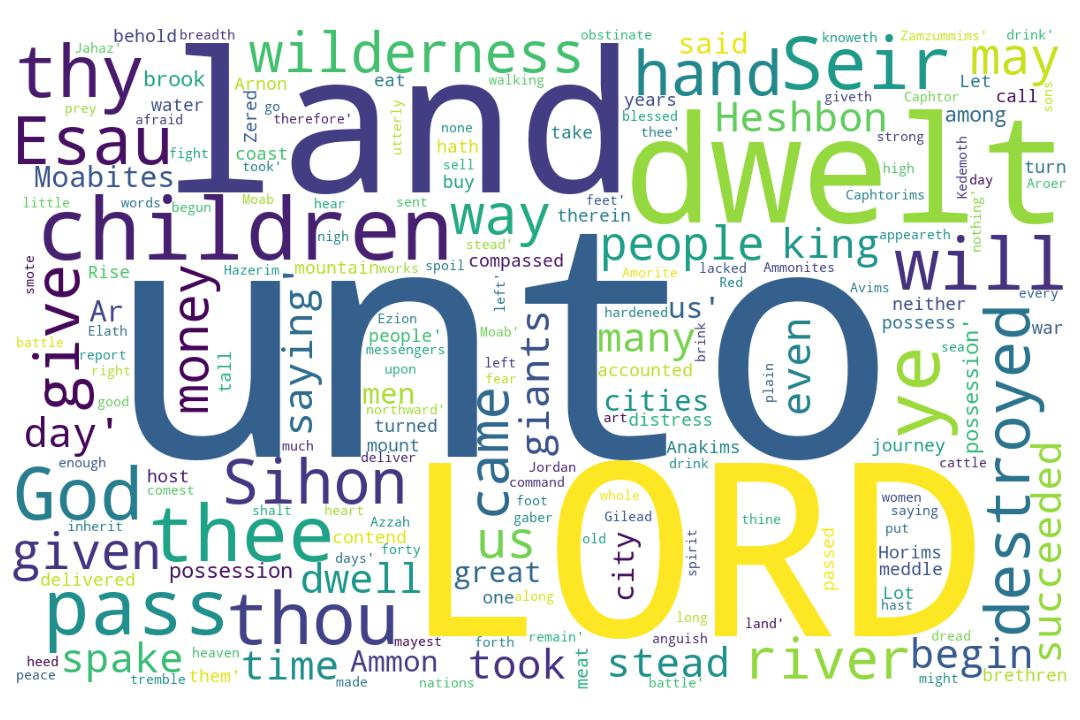
\includegraphics[width=\linewidth]{05OT-Deuteronomy/Deuteronomy2-WordCloud.jpg}
  \caption{Deuteronomy 2 Word Cloud}
  \label{fig:Deuteronomy 2 word Cloud}
\end{figure}


\marginpar{\scriptsize \centering \fcolorbox{bone}{lime}{\textbf{THE WAIT IS OVER}}\\ (Deuteronomy 2:1-37) \begin{compactenum}[I.][8]
    \item   \textbf{Wilderness} \index[scripture]{Deuteronomy!Deu 02:01}\index[scripture]{Deuteronomy!Deu 02:07}\index[scripture]{Deuteronomy!Deu 02:08}\index[scripture]{Deuteronomy!Deu 02:26} (Deu 2:1, 7, 8, 26)
    \item  \textbf{Wanderings} 
    \item  \textbf{Wait} Over \index[scripture]{Deuteronomy!Deu 02:03} (Deu 2:3)
    \item  The \textbf{Walk} \index[scripture]{Deuteronomy!Deu 02:07} (Deu 2:7)
    \item  What God \textbf{Will} Do \index[scripture]{Deuteronomy!Deu 02:05}\index[scripture]{Deuteronomy!Deu 02:09}\index[scripture]{Deuteronomy!Deu 02:19}\index[scripture]{Deuteronomy!Deu 02:25}\index[scripture]{Deuteronomy!Deu 02:27}\index[scripture]{Deuteronomy!Deu 02:28} (Deu 2:5, 9, 19, 25, 27, 28)
    \item  A \textbf{Warning} \index[scripture]{Deuteronomy!Deu 02:09} (Deu 2:9)
    \item  The High \textbf{Way} \index[scripture]{Deuteronomy!Deu 02:27} (Deu 2:27)
\end{compactenum}}

\footnote{\textcolor[cmyk]{0.99998,1,0,0}{\hyperlink{TOC}{Return to end of Table of Contents.}}}\footnote{\href{https://audiobible.com/bible/deuteronomy_2.html}{\textcolor[cmyk]{0.99998,1,0,0}{Deuteronomy 2 Audio}}}\textcolor[cmyk]{0.99998,1,0,0}{Then we turned, and took our journey into the \fcolorbox{bone}{lime}{wilderness} by the way of the Red sea, as the LORD spake unto me: and we compassed mount Seir many days.}
[2] \textcolor[cmyk]{0.99998,1,0,0}{And the LORD spake unto me, saying,}
[3] \textcolor[cmyk]{0.99998,1,0,0}{Ye have compassed this mountain \fcolorbox{bone}{lime}{long enough}: turn you northward.}
[4] \textcolor[cmyk]{0.99998,1,0,0}{And command thou the people, saying, Ye \emph{are} to pass through the coast of your brethren the children of Esau, which dwell in Seir; and they shall be afraid of you: take ye good heed unto yourselves therefore:}
[5] \textcolor[cmyk]{0.99998,1,0,0}{Meddle not with them; for I will not give you of their land, no, not so much as a foot breadth; because \fcolorbox{bone}{lime}{I have given} mount Seir unto Esau \emph{for} a possession.}
[6] \textcolor[cmyk]{0.99998,1,0,0}{Ye shall buy meat of them for money, that ye may eat; and ye shall also buy water of them for money, that ye may drink.}
[7] \textcolor[cmyk]{0.99998,1,0,0}{For the LORD thy God hath blessed thee in all the works of thy hand: he knoweth thy \fcolorbox{bone}{lime}{walking} through this great \fcolorbox{bone}{lime}{wilderness}: these forty years the LORD thy God \emph{hath} \emph{been} with thee; thou hast lacked nothing.}
[8] \textcolor[cmyk]{0.99998,1,0,0}{And when we passed by from our brethren the children of Esau, which dwelt in Seir, through the way of the plain from Elath, and from Ezion-gaber, we turned and passed by the way of the \fcolorbox{bone}{lime}{wilderness} of Moab.}
[9] \textcolor[cmyk]{0.99998,1,0,0}{And the LORD said unto me, Distress not the Moabites, neither contend with them in battle: for \fcolorbox{bone}{lime}{I will not} give thee of their land \emph{for} a possession; because \fcolorbox{bone}{lime}{I have given} Ar unto the children of Lot \emph{for} a possession.}
[10] \textcolor[cmyk]{0.99998,1,0,0}{The Emims dwelt therein in times past, a people great, and many, and tall, as the Anakims;}
[11] \textcolor[cmyk]{0.99998,1,0,0}{Which also were accounted giants, as the Anakims; but the Moabites call them Emims.}
[12] \textcolor[cmyk]{0.99998,1,0,0}{The Horims also dwelt in Seir beforetime; but the children of Esau succeeded them, when they had destroyed them from before them, and dwelt in their stead; as Israel did unto the land of his possession, which the LORD gave unto them.}
[13] \textcolor[cmyk]{0.99998,1,0,0}{Now rise up, \emph{said} \emph{I}, and get you over the brook Zered. And we went over the brook Zered.}
[14] \textcolor[cmyk]{0.99998,1,0,0}{And the space in which we came from \fcolorbox{bone}{MYGOLD}{Kadesh-barnea}, until we were come over the brook Zered, \emph{was} thirty and eight years; until all the generation of the men of war were wasted out from among the host, as the LORD sware unto them.}
[15] \textcolor[cmyk]{0.99998,1,0,0}{For indeed the hand of the LORD was against them, to destroy them from among the host, until they were consumed.}
[16] \textcolor[cmyk]{0.99998,1,0,0}{So it came to pass, when all the men of war were consumed and dead from among the people,}
[17] \textcolor[cmyk]{0.99998,1,0,0}{That the LORD spake unto me, saying,}
[18] \textcolor[cmyk]{0.99998,1,0,0}{Thou art to pass over through Ar, the coast of Moab, this day:}
[19] \textcolor[cmyk]{0.99998,1,0,0}{And \emph{when} thou comest nigh over against the children of Ammon, distress them not, nor meddle with them: for I will not give thee of the land of the children of Ammon \emph{any} possession; because \fcolorbox{bone}{lime}{I have given} it unto the children of Lot \emph{for} a possession.}
[20] \textcolor[cmyk]{0.99998,1,0,0}{(That also was accounted a land of giants: giants dwelt therein in old time; and the Ammonites call them Zamzummims;}
[21] \textcolor[cmyk]{0.99998,1,0,0}{A people great, and many, and tall, as the Anakims; but the LORD destroyed them before them; and they succeeded them, and dwelt in their stead:}
[22] \textcolor[cmyk]{0.99998,1,0,0}{As he did to the children of Esau, which dwelt in Seir, when he destroyed the Horims from before them; and they succeeded them, and dwelt in their stead even unto this day:}
[23] \textcolor[cmyk]{0.99998,1,0,0}{And the Avims which dwelt in Hazerim, \emph{even} unto Azzah, the Caphtorims, which came forth out of Caphtor, destroyed them, and dwelt in their stead.)}\\
\\
\P \textcolor[cmyk]{0.99998,1,0,0}{Rise ye up, take your journey, and pass over the river Arnon: behold, I have given into thine hand Sihon the Amorite, king of Heshbon, and his land: begin to possess \emph{it}, and contend with him in battle.}
[25] \textcolor[cmyk]{0.99998,1,0,0}{This day \fcolorbox{bone}{lime}{will I} begin to put the dread of thee and the fear of thee upon the nations \emph{that} \emph{are} under the whole heaven, who shall hear report of thee, and shall tremble, and be in anguish because of thee.}
[26] \textcolor[cmyk]{0.99998,1,0,0}{And I sent messengers out of the wilderness of Kedemoth unto Sihon king of Heshbon with words of peace, saying,}
[27] \textcolor[cmyk]{0.99998,1,0,0}{Let me pass through thy land: \fcolorbox{bone}{lime}{I will} go along by the high way, \fcolorbox{bone}{lime}{I will} neither turn unto the right hand nor to the left.}
[28] \textcolor[cmyk]{0.99998,1,0,0}{Thou shalt sell me meat for money, that I may eat; and give me water for money, that I may drink: only \fcolorbox{bone}{lime}{I will} pass through on my feet;}
[29] \textcolor[cmyk]{0.99998,1,0,0}{(As the children of Esau which dwell in Seir, and the Moabites which dwell in Ar, did unto me;) until I shall pass over Jordan into the land which the LORD our God giveth us.}
[30] \textcolor[cmyk]{0.99998,1,0,0}{But Sihon king of Heshbon would not let us pass by him: for the LORD thy God hardened his spirit, and made his heart obstinate, that he might deliver him into thy hand, as \emph{appeareth} this day.}
[31] \textcolor[cmyk]{0.99998,1,0,0}{And the LORD said unto me, Behold, I have begun to give Sihon and his land before thee: begin to possess, that thou mayest inherit his land.}
[32] \textcolor[cmyk]{0.99998,1,0,0}{Then Sihon came out against us, he and all his people, to fight at Jahaz.}
[33] \textcolor[cmyk]{0.99998,1,0,0}{And the LORD our God delivered him before us; and we smote him, and his sons, and all his people.}
[34] \textcolor[cmyk]{0.99998,1,0,0}{And we took all his cities at that time, and utterly destroyed the men, and the women, and the little ones, of every city, we left none to remain:}
[35] \textcolor[cmyk]{0.99998,1,0,0}{Only the cattle we took for a prey unto ourselves, and the spoil of the cities which we took.}
[36] \textcolor[cmyk]{0.99998,1,0,0}{From Aroer, which \emph{is} by the brink of the river of Arnon, and \emph{from} the city that \emph{is} by the river, even unto Gilead, there was not one city too strong for us: the LORD our God delivered all unto us:}
[37] \textcolor[cmyk]{0.99998,1,0,0}{Only unto the land of the children of Ammon thou camest not, \emph{nor} unto any place of the river Jabbok, nor unto the cities in the mountains, nor unto whatsoever the LORD our God forbad us.}